\section{Considerações Finais}

Conectamos o ESP32 ao computador utilizando um cabo microUSB. Enviamos o código para o microcontrolador apertando o atalho \textit{Alt + Ctrl + U} no VSCode. Feito o envio, é necessário apertar o botão EN para que ele comece a funcionar.

Como é a primeira vez, será exibido no monitor que não foi possível conectar à uma rede Wi-Fi. Então é exibido um endereço IP para acessar-mos no computador ou pelo celular. Antes, é necessário conectar o dispositivo ao \textit{access point} do ESP32. Por padrão, ele é "ESP-Wifi-Manager", mas ele pode ser alterado no método \textit{softAP}.

Após conectado, acessamos o endereço IP pelo browser e nos é apresentado o formulário para preencher com as credenciais de alguma rede disponível. E submetemos o formulário, para então sermos direcionados a outra página informando que o ESP32 será resetado. Ao reiniciar, a página exibida será a \textit{index}.

\begin{figure}[H]
    \centering
    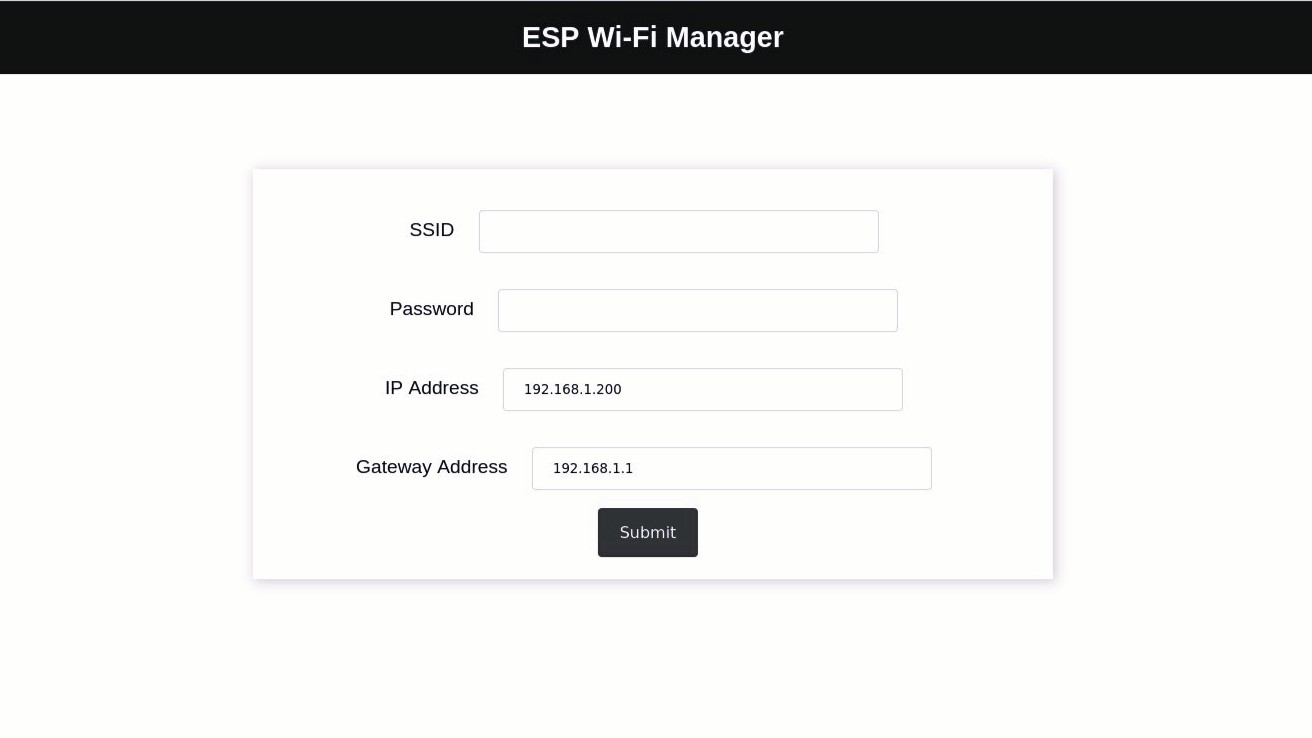
\includegraphics[width=0.5\linewidth]{img/screen.jpg}
    \caption{Formulário de credenciais.}
    \label{fig:credentials}
\end{figure}

É possível conferir o código completo nesse \href{https://github.com/fabricio-araujo94/microcontroladores/tree/main/wifi_manager_}{repositório} no GitHUb.